\section{Elliptiske kurver}

Elliptiske kurver er en familie kurver som også har egenskapen at de danner grupper
under en gitt gruppe-operator.
\cite{silverman_arithmetic_2009}

\subsection{Komplekse elliptiske kurver}
\begin{definition}
    En undergruppe $\Lambda\subset \mathbb C$ er et \textit{gitter}
    dersom det kan skrives som bildet av en morfi $\phi\colon \mathbb Z^2\to \mathbb C$.
    Det er av \textit{full rang} om $\phi$ er injektiv
    og $\phi(e_1) / \phi(e_2)\notin \mathbb R$.
\end{definition}

Et gitter er unikt definert av to punkter $\omega_1, \omega_2\in \mathbb C$,
ved å la $\phi$ være morfien $e_1\mapsto \omega_1$, $e_2\mapsto \omega_2$,
så gitteret $\Lambda = \langle \omega_1, \omega_2\rangle$.
Men flere ulike valg av $\omega_1, \omega_2$ gir samme elliptiske kurve.
Til eksempel er $\langle 1, i\rangle = \langle 1, 1 + i\rangle$.
\begin{figure}[htb]
    \centering
    \begin{tikzpicture}
        \foreach \x in {-2,...,2}
        \foreach \y in {-2,...,2}
        {
            \fill (\x, \y) circle (1pt);
        }
        \draw[->] (-2, 0) -- (2,0)
            node[right]{$\mathbb R$};
        \draw[->] (0, -2) -- (0, 2)
            node[above right]{$i\mathbb R$};
        \draw[->, thick] (0,0) -- (1,0)
            node[above right]{$\omega_1=1$};
        \draw[->, thick] (0,0) -- (1,1)
            node[above right]{$\omega_2=1 + i$};
    \end{tikzpicture}
    \caption{Gitteret $\Lambda = \langle 1, 1 + i\rangle$.}
\end{figure}

På samme måte som vi kan konstruere enhetsirkelen som restgruppen
\[
    0
    \to \langle 1\rangle
    \to \mathbb R
    \mathbb S^1
    \to 1
\]
så kan vi se på restgruppen $\mathbb C / \Lambda$
som en torus
\[
    0
    \to \Lambda
    \to \mathbb C
    \to S^1\times S^1
    \to 1.
\]
En torus er et eksempel på en genus $1$ flate,
fordi den har ett ``hull'',
men når vi konstruerer det som et kvotient av $\mathbb C$
får den noe struktur i likhet med strukturen på $\mathbb C$
som skiller den fra $\mathbb R^2$.
Spesielt bør vi tenke på $\mathbb C / \Lambda$ som noe av
samme ``komplekse'' dimensjon som $\mathbb C$,
altså $1$.
Dermed ser vi på $\mathbb C / \Lambda$ som en kurve av genus $1$,
heller enn som en flate.



\subsection{Reelle elliptiske kurver}

En kompleks elliptisk kurve kan også avbildes inn i det komplekse planet,
på en slik måte at vi kan gjenkjenne gruppestrukturen til kurven.
Spesielt kan alle kurvene skrives som løsningsmengden til en likning på formen
\begin{equation}\label{eq:weierstrass}
    y^2 = x^3 + Ax + B
\end{equation}
for tall $A,B\in \mathbb C$.
Denne likningen kalles \textit{Weierstrass likningen}
\cite[p.~45]{silverman_arithmetic_2009}.

Det komplekse planet er av reell dimensjon $4$,
så for å forstå hvordan gruppestrukturen til kurven er bevart
kan vi restriktere til de løsningene av \cref{eq:weierstrass}
hvor $x,y\in \mathbb R$ og $A,B\in \mathbb R$.
Dette gir oss reelle elliptiske kurver.

\begin{figure}[htb]
    \centering
    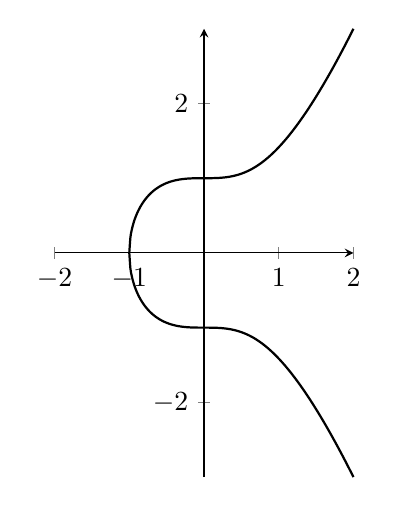
\begin{tikzpicture}
        \begin{axis}[
                xmin=-2,
                xmax=2,
                ymin=-3,
                ymax=3,
                domain=-1:2,
                samples=200,
                axis lines=middle,
                clip=false,
                axis equal image=true,
                smooth=true,
            ]
            \addplot[black, thick]{sqrt(x^3 + 1)};
            \addplot[black, thick]{-sqrt(x^3 + 1)};
        \end{axis}
    \end{tikzpicture}
    \caption{Løsningsmengden $\{y^2 = x^3 + 1\}\subset \mathbb R^2$.}
\end{figure}

La $C\subset \mathbb R^2$ være en elliptisk kurve,
og la $P, Q\in C$ være to punkter på kurven.
For å regne ut summen trekker vi en linje $l$ mellom $P$ og $Q$,
eller om $P = Q$ tar vi tangenten til $C$ i $P$.
Ved Bezouts teorem finnes det et tredje punkt $R\in C\cap l$,
med $R\neq P,Q$.
Vi definerer speilingen av $R$ om $x$-aksen $-R = P + Q$.

\begin{figure}[htb]
    \centering
    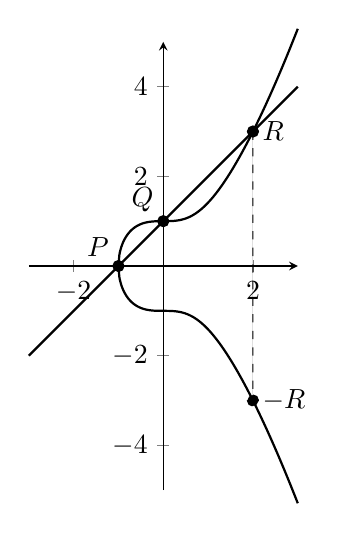
\begin{tikzpicture}
        \begin{axis}[
                xmin=-3,
                xmax=3,
                ymin=-5,
                ymax=5,
                axis lines=middle,
                clip=false,
                axis equal image=true,
            ]
            \addplot[
                black,
                thick,
                domain=-1:3,
                samples=200,
                smooth=true,
            ]{sqrt(x^3 + 1)};
            \addplot[
                black,
                thick,
                domain=-1:3,
                samples=200,
                smooth=true,
            ]{-sqrt(x^3 + 1)};
            \addplot[
                black,
                thick,
                domain=-3:3,
            ]{x + 1};
            \pgfplotsextra{
                \draw (axis cs:-1, 0) circle (2pt)[fill]
                    node[above left] {$P$};
                \draw (axis cs:0, 1) circle (2pt)[fill]
                    node[above left] {$Q$};
                \draw (axis cs:2, 3) circle (2pt)[fill]
                    node[right] {$R$};
                \draw[dashed] (axis cs:2, 3) -- (axis cs:2, -3)
                    circle (2pt)[fill]
                    node[right] {$-R$};
            }
        \end{axis}
    \end{tikzpicture}
\end{figure}

Ekvivalent sier vi at om tre punkter $P,Q,R$ ligger på samme linje
så er $P + Q + R = 0$.
Merk at for at Bezout skal holde må vi i teorien regne med punkter som ligger
i ``uendeligheten''.
Dette oppstår nøyaktig når vi velger punkter $P,Q$ som er speilingen
av hverandre om $x$-aksen,
altså når $P = -Q$.
For vår kurve finnes det bare ett punkt i uendeligheten, og dette kaller vi $\infty$.
Merk at $\infty$ er identitetselementet i gruppen.

\subsection{Elliptiske kurver over $\mathbb Z / n$}

Husk at for en gruppe $\mathbb Z / n$ kan vi i tillegg definere
multiplikasjon $\mu\colon (\mathbb Z / n)\times (\mathbb Z / n)\to \mathbb Z / n$.
Multiplikasjon oppfører seg ganske likt som multiplikasjon på til eksempel
$\mathbb R$.
Spesielt har vi at $(a + b)c = ac + bc$.

Siden vi kan snakke om både multiplikasjon og addisjon på $\mathbb Z / n$,
gir det også mening å definere polynomer for $\mathbb Z / n$,
så vi kan til eksempel finne løsninger til likningen
\[
    y^2 = x^3 + Ax + B
\]
i ${(\mathbb Z / n)}^2$ om vi lar $A, B\in \mathbb Z / n$.

Tilsvarende kan vi definere en linje i ${(\mathbb Z / n)}^2$
som løsningsnmengden av en likning på formen
\[
    ax + by = c,
\]
og om vi velger $n = p$ et primtall kan vi igjen forvente å finne
tre punkter i skjæringen
\[
    \{y^2 = x^3 + Ax + B\}\cap \{ax + by = c\}.
\]

\begin{figure}
    \centering
    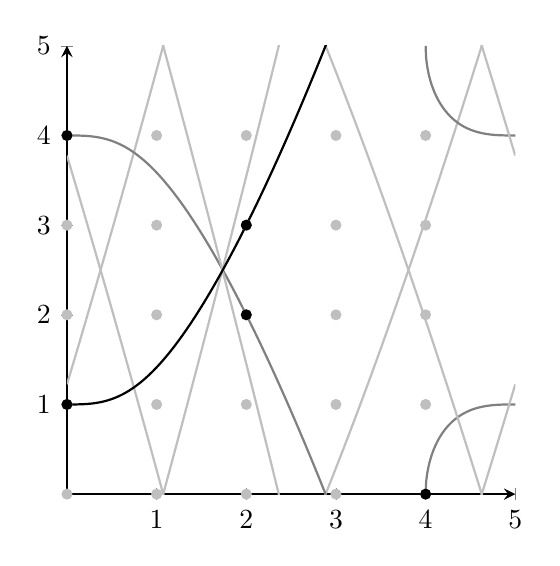
\begin{tikzpicture}
        \begin{axis}[
                xmin=0,
                xmax=5,
                ymin=0,
                ymax=5,
                axis lines=middle,
                axis equal image=true,
                samples=200,
                smooth=true,
                thick,
                clip=false,
            ]
            \begin{scope}
                \clip (axis cs:0,0) -- (axis cs:5,0)
                    -- (axis cs:5,5)
                    -- (axis cs:0,5)
                    -- cycle;
                % Above
                \addplot[
                    gray,
                    domain=4:5
                ]{sqrt((x - 5)^3 + 1)};
                \addplot[
                    lightgray,
                    domain=2.5:5,
                ]{sqrt(x^3 + 1) - 5};
                \addplot[
                    lightgray,
                    domain=4:5
                ]{sqrt(x^3 + 1) - 10};
                \addplot[
                    lightgray,
                    domain=0:1.5
                ]{sqrt((x + 5)^3 + 1) - 10};
                \addplot[
                    lightgray,
                    domain=1:2.5
                ]{sqrt((x + 5)^3 + 1) - 15};
                % Below
                \addplot[
                    gray,
                    domain=4:5
                ]{5 - sqrt((x - 5)^3 + 1)};
                \addplot[
                    gray,
                    domain=0:3,
                ]{5 - sqrt(x^3 + 1)};
                \addplot[
                    lightgray,
                    domain=2.5:5,
                ]{10 - sqrt(x^3 + 1)};
                \addplot[
                    lightgray,
                    domain=4:5
                ]{15 - sqrt(x^3 + 1)};
                \addplot[
                    lightgray,
                    domain=0:1.5
                ]{15 - sqrt((x + 5)^3 + 1)};
                \addplot[
                    lightgray,
                    domain=1:2.5
                ]{20 - sqrt((x + 5)^3 + 1)};
                % Main
                \addplot[
                    black,
                    domain=0:3,
                ]{sqrt(x^3 + 1)};
            \end{scope}
            \pgfplotsextra{
                \foreach \x in {0,...,4}
                \foreach \y in {0,...,4}
                {
                    \fill[lightgray] (axis cs:\x, \y) circle (2pt);
                }
                \foreach \x/\y in {0/1, 0/4, 2/3, 2/2, 4/0}
                {
                    \fill[black] (axis cs:\x, \y) circle(2pt);
                }
            }
        \end{axis}
    \end{tikzpicture}
\end{figure}

\subsection{Elliptiske kurver i kryptografi}
La nå $n = p$ være et primtall (eller en potens av et primtall)
og $C\subset \mathbb {(Z / p)}^2$
være en elliptisk kurve på Weierstrass form.
Siden $\#{(Z / p)}^2 = p^2$ er endelig må også $\#C$ være endelig,
altså en endelig (abelsk) gruppe.

Et resultat kjent som Hasses teorem \cite[Thm.~V.1.1]{silverman_arithmetic_2009}
gir oss et grovt estimat på $\#C$.
Det forteller oss at
\[
    \left|
        \# C - p - 1
    \right| \leq 2 \sqrt p,
\]
altså forventer vi omtrent $p$ punkter på $C$,
så om vi kan konstruere kurver slik at $\#C$
har store primtallsfaktorer har vi en erstatning
for ${(\mathbb Z / p)}^\times$ som er minst like god for beregning av
til eksempel Diffie-Hellman.

\todo[inline]{Siter indeks kalkulus for hvorfor vi foretrekker elliptiske kurver.}
